\section{Method}

TODO introductionary paragraph

\subsection{Test Data}

The first important step is to create a test data set to run the evaluations with and verify them.

TODO explain the source and structrue

\subsection{Clustering method}

Clustering finds similarities in different news articles based on their content and groups them together, while unrelated news are regarded as noise. The challenge now araises to find an appropriate clustering method, which is able to work with data of varying densities and of high dimensionality.

TODO why hdbscan

\subsubsection{HDBSCAN}

HDBSCAN is a hierarchical density-based clustering algorithm \cite{McInnes2017}. It extends the well known [insert citation] DBSCAN algorithm and reduces its sensitivity for clusters of varying densities. Another important quality of HDBSCAN is, that it does not need to know the number of clusters up front.

 TODO explain some more

\subsubsection{K-means}

KMeans is a centroid-based clustering algorithm. 

 TODO explain some more

\subsubsection{Preprocessing}

% raw text
% with entity extraction
% word embeddings?
% Tfidf

\subsubsection{Scoring function}

The scoring function is essential for measuring the result of a clustering method. The score should reflect the quality of the individual clusters and of the clustering as a whole. The number of existing measures for clustering is vast and can be split into two main categories. Internal measures determine the score based on criteria derived from the data itself and external measures depend on criteria non-existent in the data itself such as class labels. Since the ground truth is known in our test data, we are going to apply an external measure.   
Initially we used Normalized Mutual Information (NMI) as our primary scoring function. The NMI is a entropy-based measure and tries to quantify the amount shared information between the clusterings. The score proved to work well for our initial evaluations, but upon closer inspection certain anomalies were found. An example is given in table \ref{tab:nmi_kmeans_example}, where K-means achieved a rather high score, regardless of the significant difference between the true amount of clusters and the approximation using $\sqrt{n}$.

% TODO explain the reason for the big difference

TODO add number of estimated clusters
\begin{table}[h]
    \centering
    \begin{tabular}{|l|l|l|l|l|}
    \hline
    \textbf{Algorithm} & \textbf{Sample Size} & \textbf{NMI}  & $\mathbf{n_{true}}$ & $\mathbf{ \mid n_{true} - n_{predicted} \mid }$ \\ \hline
    k-means & 19255 & 0.754 & 600 & 457 \\ \hline
    hdbscan & 19255 & 0.742 & 600 & 2 \\ \hline
    \end{tabular}
    \caption{K-Means has a higher NMI score than HDBSCAN, while having a much larger difference in number of clusters.}
    \label{tab:nmi_kmeans_example}
\end{table}

Other scoring functions such as V-Measure or the Adjusted Rand Index showed similar unexpected results with different clusterings. Therefore we decided to develop our own scoring function based on the ideas of Maximum Matching and the jaccard index. 

TODO find citations

\paragraph{Calculating the score}

The scoring function first calculates the similarity between pairs of clusters, where each cluster belongs to a different clustering. We use the jaccard index to measure the similarity, which is defined as

\begin{equation}
    \label{equ:similarity}
    \frac{|A \cap B|}{|A \cup B|}
\end{equation}

To illustrate the process we start with an example. We use $T$ and $C$ as our clusterings, where $T$ is the ground truth and $C$ is the predicted clustering. The clusterings are defined as follows:

\begin{gather*}
    T = \{\{1,2,3\},\{4,5,6,7\},\{8,9\}\} \\
    C = \{\{1,2\},\{3,4,5,6\},\{7\},\{8,9\}\}
\end{gather*}

We calculate the similarity as defined in Equation \ref{equ:similarity}, for each possible pair between $T$ and $C$ starting with $t_1= \{1,2,3\}$ and $c_1 = \{1,2\}$:

\begin{align*}
    similarity(t_1,c_1) &=\frac{|t_1 \cap c_1|}{|t_1 \cup c_1|} 
    = \frac{|\{1,2\}|}{|\{1,2,3\}|} 
    = \frac{2}{3} = 0.667 \\
\end{align*}

After doing this for each possible pair we get the similarity matrix $A$:

\begin{gather*}
\begin{array}{rcl}
    A = & \left(\begin{array}{cccc}
        similarity(t_1,c_1) & \hdots & \hdots & similarity(t_1,c_4)\\
        \vdots & \vdots & \vdots & \vdots\\
        similarity(t_3,c_3) & \hdots & \hdots & similarity(t_3,c_4) \end{array}\right)
        = & \left(\begin{array}{cccc}
            0.667 & 0.167 & 0 & 0 \\
            0 & 0.6 & 0.25 & 0.4 \\
            0 &  0 & 0 & 1.0 \end{array}\right)
\end{array}
\end{gather*}

As a next step we have to select the most relevant similarity values from each row of the similarity matrix. 

Finding relevant values in the similarity matrix non-trivial, since clusters do not share labels across different clusterings. To solve this, we make two assumptions:
\begin{enumerate} 
\item The higher the similarity between two clusters, the more likely it is, that both clusters are describing the same group of documents. 
\item Each cluster can be associated with a cluster from another clustering only once.
\end{enumerate}

Based on those assumptions we select the highest similarity value per row, whose column is not already associated with another row. Applying this selection function $f$ to our previously calculated similarity matrix $A$ results in the set containing the most relevant similarity values.

\begin{gather*}
    \begin{array}{rcl}
        f(A) = & \left(\begin{array}{cccc}
            \mathbf{0.667} & 0.167 & 0 & 0 \\
            0 & \mathbf{0.6} & 0.25 & 0.4 \\
            0 &  0 & 0 & \mathbf{1.0} \end{array}\right)
            = \{0.667, 0.6, 1\}
    \end{array}
\end{gather*}

As we can see, there were no collisions between columns and we simply get the highest value per row. Consider the following example with an similarity matrix $B$, which does contain a collision:

\begin{gather*}
    \begin{array}{rcl}
        f(B) = & \left(\begin{array}{cccc}
            \mathbf{0.75} & 0.375 & 0.427 & 0.375 \\
            0.4 & \mathbf{0.667} & 0.571 & \textcolor{red}{0.8} \\
            0.333 &  0.25 & 0.4 & \mathbf{1.0} \end{array}\right)
            = \{0.75, 0.667, 1\}
    \end{array}
\end{gather*}

The selected similarity for the second row is 0.667 instead of 0.8. This is because the fourth column is already associated with the third row, while having an similarity greater than 0.8. Therefore based on our assumption that clusters cannot be associated twice, the second highest similarity is used for the second column. In case no association could be found, the value would be set to zero. The full algorithm for the selection process can be found in the appendix as listing \ref{lst:select_max_values}.

As a third step we have to calculate the weights to be used for the final  The weight is based on the number of elements inside the cluster and necessary to represent differences in predicted and true number of clusters in the final score. It is defined as follows

\begin{equation}
    \label{equ:weight}
        w_{ij} = \frac{|t_i| + |c_j|}{|T|+|C|} \\
\end{equation}

where $T$ is the ground truth with $t_i \in T$ and $C$ the predicted clustering with  $c_j \in C$. Therefore the weight for a pairing $t_ic_j$ includes both the size of the true cluster and the size of the predicted cluster. The reason both sizes are used, is that we want to reflect if the overall number of predicted clusters is different from the ground truth. Using only the true number of elements as the weight, would affect the score if |C| < |T|, but not |C| > |T|. Therefore the number of predicted elements has to be included as well. 

In the fourth and final step we calculate the weighted average, $S$ is the similarity matrix with $s_{i} \in S$

\begin{equation}
    \label{equ:weighted_average}
        \text{MP-Score} = \sum_{i=0}^{|S|} w_is_i
\end{equation}

Where $S$ is the similarity matrix with $s_{i} \in S$ and $w_i$ the corresponding weight. Using our previously selected similarity values $S = f(A) = \{0.667, 0.6, 1\}$ with  $c_{true}=3$ and $c_{predicted}=4$, the calculation for the final average would be done as follows:

\begin{align*}
    score &= \frac{\sum_{i=1}^{|S|} S_i}{c_{true} + max(0, c_{predicted} - c_{true})} \\
    &= \frac{0.667 + 0.6 + 1}{3 + max(0, 4 - 3)} = \frac{2.267}{3 + max(0, 1)} \\
    &= \frac{2.267}{3 + 1} = \frac{2.267}{4} \\
    &= \mathbf{0.567}
\end{align*}

The final score for the evaluation of the predicted cluster $C$ with the true cluster is 0.567.

\paragraph{Comparison against other measures}

The test scenarios in table \ref{tab:score_scenarios} show the resulting scores of our similarity score, NMI and completeness. It is important to note that NMI and completeness work with cluster labels assigned to each document, instead of considing elements inside a single cluster. This means the clustering will be flattened into one dimension, where each document is assigned the label of the cluster it appeares in. The array containing the labels for the first scenario would look as follows: $C=[1,1,1,2,2,2,2,3,3]$.

\begin{table}[h]
    \centering
    \begin{tabular}{|l|l|l|l|l|}
    \hline
    \multicolumn{5}{ |c| }{\textbf{Test scenarios with ground truth $T = \{\{1,2,3\},\{4,5,6,7\},\{8,9\}\}$}} \\
    \hline
    Nr. & Predicted Clustering $C$ & NMI & ARI & MP-Score \\ \hline
    1 & $C = \{\{1,2,3\},\{4,5,6,7\},\{8,9\}\}$ & 1.0 & 1.0 & 1.0 \\ \hline
    2 & $C = \{\{1,2\},\{3,4,5,6\},\{7,8,9\}\}$ & 0.564 &  0.308 & 0.637 \\ \hline
    3 & $C = \{\{1,2,3\},\{4,5,6\},\{7\},\{8,9\}\}$ & 0.895 & 0.771 & 0.847 \\ \hline
    4 & $C = \{\{1,2,3\},\{4,5\},\{6,7\},\{8\},\{9\}\}$ & 0.821 & 0.591 & 0.583 \\ \hline
    5 & $C = \{\{1\},\{2\},\{3\},\{4\},\{5\},\{6\},\{7\},\{8\},\{9\}\}$ & 0.651 & 0 & 0.227 \\ \hline
    6 & $C = \{\{1,2,3,4,5\},\{6,7,8,9\}\}$ & 0.434 & 0.182 & 0.433 \\ \hline
    7 & $C = \{\{1,2,3,4,5,6,7,8,9\}\}$ & 0.0 & 0 & 0.321 \\ \hline
    8 & $C = \{\{7,2,4\},\{8,9,6,3\},\{1,5\}\}$ & 0.219 & -0.108 & 0.392 \\ \hline
    \end{tabular}
    \caption{Direct comparison of different scoring functions}
    \label{tab:score_scenarios}
\end{table}

As a final note, repeating the evaluation shown in table \ref{tab:nmi_kmeans_example} a second time using the MP-Score, the score (Table \ref{tab:avg_predict_kmeans_example}) for K-means is much lower than HDBSCAN. This reflects what we would expect based on the big difference in the amount of predicted clusters.

\begin{table}[h]
    \centering
    \begin{tabular}{|l|l|l|l|l|}
    \hline
    \textbf{Algorithm} & \textbf{Sample Size} & \textbf{Similarity}  & $\mathbf{n_{true}}$ & $\mathbf{ \mid n_{true} - n_{predicted} \mid }$ \\ \hline
    k-means & 19255 & 0.137 & 600 & 457 \\ \hline
    hdbscan & 19255 & 0.605 & 600 & 2 \\ \hline
    \end{tabular}
    \caption{The similarty score reflects the difference in number of predicted clusters.}
    \label{tab:avg_predict_kmeans_example}
\end{table}

\subsection{Online Clustering}

Detecting events in a stream of news articles will be achieved by using an online clustering approach. The events of interest for this application are the discovery of new topics and the extension of existing topics. Thus we define our two events as follows:

\begin{itemize}
    \item Topic added: A new cluster of news articles appears in the data stream.
    \item Topic extended: An existing topic is extended by additional news articles.
\end{itemize}

HDBSCAN will be applied as the clustering method, using the optimal settings as discovered in the preivous evaluation. Additional preprocessing of news articles before clustering is going to be explored as part of evaluation as well and will be implemented accordingly for the online clustring.

Since HDBSCAN only supports static datasets, the clustering will be done in batches using a time based sliding window approach. Events are detected by comparing the resulting clusters with the previous ones.

\begin{figure}[h]
    \centering

    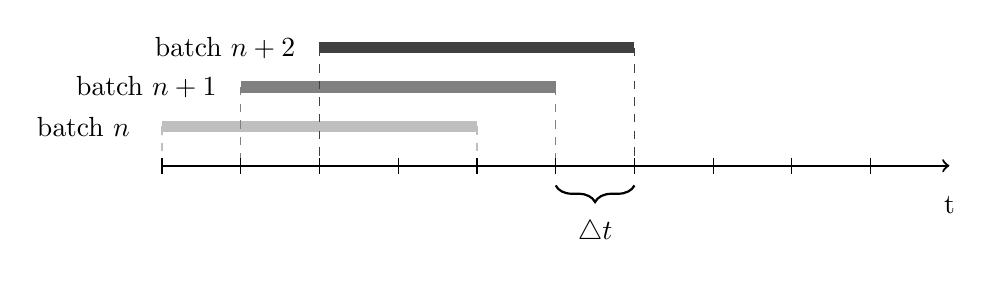
\begin{tikzpicture}[scale=1]
        
       
        \draw[lightgray, line width=4pt] (0,.5) -- (4,.5);
        \draw[lightgray, dashed] (0,.5) -- (0,0);
        \draw[lightgray, dashed] (4,.5) -- (4,0);
        \node[align=right] at (-1,.5) {batch $n$};

        \draw[gray, line width=4pt] (1,1) -- (5,1);
        \draw[gray, dashed] (1,1) -- (1,0);
        \draw[gray, dashed] (5,1) -- (5,0);
        \node[align=right] at (-.2,1) {batch $n + 1$};

        \draw[darkgray, line width=4pt] (2,1.5) -- (6,1.5);
        \draw[darkgray, dashed] (2,1.5) -- (2,0);
        \draw[darkgray, dashed] (6,1.5) -- (6,0);
        \node[align=right] at (0.8,1.5) {batch $n + 2$};

        \node[align=center] at (5.5,-0.85) {$\triangle t$};
        \node[align=center] at (10,-0.5) {t};

        \draw [thick,->] (0,0) -- (10,0);
        \foreach \x in {0,...,9} \draw (\x,0.1) -- (\x,-0.1);

        \draw [thick,decorate,decoration={brace,amplitude=6pt,raise=0pt,mirror}] (5,-0.25) -- (6,-0.25);

        \end{tikzpicture}
        
    \caption{Timeline showing the sliding window approach}
    \label{fig:timeline}
\end{figure}

\subsubsection{Finding pairs clusters}

To be able to compare clusters of different batches with each other, we have to find pairs of clusters between batches, which describe the same topic. This is done by applying the same assumptions as for the scoring function used in the evaluation. Therefore clusters are paired based on their similarity calculated with the jaccard index as shown in equation \ref{equ:similarity}. If the similarity is above a certain threshold, both clusters are seen as describing the same topic.

\subsubsection{Sliding window}

An important consideration for determining existing or new clusters is the overlap of samples between batches. If the overlap is too small, similar clusters will no longer be detected as such, which would result in an increasingly high error rate. Finding optimal values for the step size between batches and the number of samples for each batch is therefore essential for our online clustering approach.